\documentclass[xcolor=dvipsnames]{beamer}
%\documentclass[handout,xcolor=dvipsnames,pdftex,hyperref={colorlinks=false}]{beamer}

% == Packages for beamer
\usepackage{xcolor}
\usepackage{graphicx}
\usepackage{fancybox}
\usepackage{hyperref}
\usepackage{amsmath,amssymb,amsfonts,bm}
\usepackage{wasysym}

\usepackage[english]{babel}
\usepackage{times}
\usepackage[T1]{fontenc}

% == Other Packages
\usepackage{rotating}
\usepackage{latexsym}
\usepackage{ulem}

% == theme & colors
\usetheme{Warsaw}  % Jens' previous
\usepackage{helvet}
\definecolor{someblue}{rgb}{0,.1,0.8}

% == New Commands
% = For general typesetting
\newcommand\spacingset[1]{\renewcommand{\baselinestretch}{#1}\small\normalsize}
\renewcommand\r{\right}
\renewcommand\l{\left}

\newcommand\makegaps{\addtolength{\itemsep}{.25\baselineskip}}
\newcommand\makebiggaps{\addtolength{\itemsep}{.5\baselineskip}}

% = For stats & econometrics
\renewcommand{\epsilon}{\varepsilon}
\newcommand\ud{\mathrm{d}}
\newcommand\dist{\buildrel\rm d\over\sim}
\newcommand\ind{\stackrel{\rm indep.}{\sim}}
\newcommand\iid{\stackrel{\rm i.i.d.}{\sim}}
\newcommand\logit{{\rm logit}}
\newcommand\cA{\mathcal{A}}
\newcommand\cN{\mathcal{N}}
\newcommand\E{\mathbb{E}}
\newcommand\V{\mathbb{V}}
\newcommand\cJ{\mathcal{J}}
\newcommand\y{{\bm y}}
\newcommand\Y{{\bm Y}}
\newcommand\X{{\bm X}}
\newcommand\x{{\bm x}}
\newcommand\eps{{\bm\varepsilon}}
\newcommand\zero{{\bm 0}}
\newcommand\be{{\bm\beta}}
\renewcommand\b{{\bm b}}
\newcommand\C{{\bm C}}
\newcommand\D{{\bm D}}
\newcommand\I{{\bm I}}
\newcommand\Z{{\bm Z}}
\newcommand\eeta{{\bm \eta}}
\DeclareMathOperator*\plim{plim}
\DeclareMathOperator\rank{rank}
\newcommand\indep{\protect\mathpalette{\protect\independenT}{\perp}}
\DeclareMathOperator{\sgn}{sgn}
\def\independenT#1#2{\mathrel{\rlap{$#1#2$}\mkern2mu{#1#2}}}

\def\therefore{{\tiny$\bullet$}\kern-0.2ex\raisebox{1ex}{\tiny$\bullet$}\kern-0.2ex{\tiny$\bullet$}}

%\newcommand{\indep}{{\bot\negthickspace\negthickspace\bot}}
\newcommand{\notindep}{{\bot\negthickspace\negthickspace\bot}{\negthinspace
  \negmedspace \negthickspace \negthickspace \diagup
  \;}}

\newcommand{\bs}{\boldsymbol}
\newcommand{\mb}{\mathbf}
\newcommand{\real}{\mathbb{R}}
\renewcommand{\u}{\ensuremath{\mb{u}}}
\renewcommand{\v}{\ensuremath{\mb{v}}}
\newcommand{\U}{\ensuremath{\mb{U}}}
\newcommand{\M}{\ensuremath{\mb{M}}}
\renewcommand{\b}{\ensuremath{\bs{\beta}}}
\newcommand{\e}{\ensuremath{\bs{\epsilon}}}
\newcommand{\bhat}{\ensuremath{\hat{\bs{\beta}}}}
\newcommand{\XX}{\ensuremath{\X'\X}}
\newcommand{\XXinv}{\ensuremath{\left(\XX\right)^{-1}}}
\newcommand{\hatsig}{\ensuremath{\hat{\sigma}^2}}
\newcommand{\sig}{\ensuremath{\sigma^2}}
\newcommand{\hatmat}{\ensuremath{\X \XXinv \X'}}
\newcommand{\ehat}{\ensuremath{\hat{\e}}}
\newcommand{\tr}{\text{tr}}
\newcommand{\Sig}{\ensuremath{\bs{\Sigma}}}
\newcommand{\SigInv}{\ensuremath{\bs{\Sigma^{-1}}}}
\newcommand{\W}{\ensuremath{\mb{W}}}

\title[]{PS200C Causal Inference, Spring 2026}
\subtitle[ ]{Introduction}
\author[Hazlett]{Chad Hazlett }
\institute[UCLA]{UCLA\\[1ex]
  \texttt{chazlett@ucla.edu}
}
\date{}

\definecolor{dgreen}{rgb}{0,.6,0.8}
\newtheorem{assumption}{Assumption}
\useoutertheme{infolines}
\begin{document}

\subject{Talks}
\AtBeginSection[]
{
  \begin{frame}<beamer>
    \frametitle{Outline}
    \tableofcontents[currentsection]
  \end{frame}
}

\AtBeginSubsection[]
{
  \begin{frame}<beamer>
    \frametitle{Outline}
    \tableofcontents[currentsection,currentsubsection]
  \end{frame}
}

\begin{frame}
  \titlepage
\end{frame}


\begin{frame}
\frametitle{Modes of Statistical Inference}
  \begin{enumerate}
  \item[1.] Descriptive Inference: summarizing and exploring data
    \begin{itemize}
    \item means, correlations, regression coefficients
    \item hypothesis testing
    \item inferring ``ideal points'' from roll-call votes
    \item inferring ``topics'' from texts and speeches
    \end{itemize}
    \medskip \pause
  \item[2.] Predictive Inference: forecasting out-of-sample data
    points
    \begin{itemize}
    \item predicting future state failures from past failures and covariates
    \item predicting vote share from a survey of likely-voters
   \end{itemize}

    \medskip \pause
  \item[3.] \alert{Causal Inference}: engages {\it counterfactuals}
    \begin{itemize}
    \item inferring whether the lack of war among democracies can be attributed to regime type
    \item determining whether a medical treatment improved outcomes.
    \item generally, estimating effect of some policy or institution or treatment on some outcome...
    \end{itemize}
  \end{enumerate}

\end{frame}

\begin{frame}{You cannot escape}

Actually it's more than that,
\small

\begin{enumerate}
\item \textit{Some} descriptive enterprises are truly descriptive, but many are at least hoping the reader thinks the result is ``suggestive'' or ``consistent with'' a causal implication.
\medskip
\item Issues such as missingness, case-selection, choosing what to condition on, and generalization all actually invoke causal assumptions, even if your goals are descriptive.
\medskip
\item If you can do a randomized experiment, great, but many questions (e.g. mediation) aren't answered by the randomization.
\end{enumerate}
\end{frame}

\begin{frame}{Is causal inference more difficult?}
\onslide<1-> Version 1: Is it more difficult as a scientific problem?\\
\small
\begin{itemize}
\item Yes.
\item Why? Because the assumptions required to say things about unobervable counterfactuals are understandably onerous.
\end{itemize}
\medskip
\normalsize
\onslide<2-> Version 2: Is it more difficult to \textit{learn and do}?\\
\small
\begin{itemize}
\item Yes and no.
\item \textcolor{blue}{Yes}: it is a different way of thinking that may be awkward and magical sounding at first!
\item \textcolor{blue}{No}: the challenges are conceptual, not technical or mathematical.
\end{itemize}
\small
\onslide<3-> In fact, I hope the course helps to convince you that technical sophistication of methods often does not solve core problems...its not about the latest estimator, machine learning, or more complicated standard errors.
\end{frame}


\begin{frame}{Causal inference $\neq$ data analysis}
\small
\onslide<1-> The shift in thinking needed for this course begins by \textbf{getting away from the idea that data ``speak for themselves''.} Data $\neq$ evidence. \\
\medskip
\onslide<2-> Rather, there are causal quantities you'd like to know, but \textit{without further assumptions}, data are largely silent on them, no matter how much you have. \\
\medskip
\onslide<3->
Stylized illustration:
\begin{itemize}
\item you have data on X and Y
\item you want to learn some effect of X on Y
\item you compute something with data, say, $coef(Y\sim X)$
\item trust me (for now): \textit{without further assumption}, any causal effect can produce any coefficient...and thus any coefficient you get is equally suggestive of any causal effect.
\end{itemize}
\onslide<3-> In other words, ``looking at the data'' is not a sufficient strategy (nor value) for learning about the world... \\
\bigskip
\onslide<4-> Curious as to what it takes? What could be better than data? Take the class!
\end{frame}


\begin{frame}
\onslide<1-> Causal inference is about that ``further assumption'' bit:
\small
\begin{itemize}
\item<2-> What assumptions can we make in order to connect the causal thing we want to know to something in the data?
\item<3-> In other words can we \textcolor{blue}{identify} our quantity of interest with something we can estimate?
\item<4-> Accordingly, we speak of \textcolor{blue}{identification assumptions} or \textcolor{blue}{identification strategies} that provide such bridges.
\end{itemize}
\normalsize
\medskip
\onslide<5-> Causal inference then is about stating the assumptions/strategies and arguing whether they are defensible
\small
\begin{itemize}
\item<6-> most identifying assumptions cannot be proven correct using data! It's not about ``knowing the right test'' to run.
\item<7-> hence we will always be appealing to information, assumptions, or context from outside the data!
\item<8-> ... it is not the method or estimator, much less software, that makes the result causal.
\end{itemize}
\end{frame}

\begin{frame}{Causal Identification Requires Assumptions}
\small
\onslide<1-> Put differently,
\bigskip
\begin{center}
Assumptions + Data $\rightarrow$ Causal Conclusions
\end{center}
\bigskip
\onslide<3-> Credibility does NOT derive from ``what method you used'' or how new it is
\begin{itemize}
\item  ...It is about finding a technique whose assumptions you can work with
\item There are not ``causal methods''!  You can't say ``it's causal because I did xyz.''
\item This is one of the hardest things for many students to absorb, in part because we are surrounded by mistakes and false advertizing.
\end{itemize}
\end{frame}

\begin{frame}{Questions Answered in This Course}
\begin{itemize}
\makebiggaps

\item<1-> Why do we accept (certain) results from randomized experiments as causal? Are they so special?

\item<2-> We often cannot run randomized experiments or want to know the effect of something that ``really happened''. Can we still make a causal inference?

\item<3-> How can we understand how vulnerable a given estimate might be to threats such as confounding?

\item<4-> \textbf{How can you conduct top quality work that seeks to make causal claims in tricky situations, while accurately characterizing what we can and cannot be claimed?}
\end{itemize}
\end{frame}

%% ============================================================
%% LOGISTICS SECTION
%% ============================================================

\begin{frame}{Approach for 2026}
\onslide<1-> This year's course reflects a deliberate shift: \\
\medskip
\small
\begin{itemize}
\item<2-> \textbf{No traditional problem sets.} AI tools can now handle much of the mechanical work---estimation, coding, debugging---that used to dominate your time outside class.
\medskip
\item<3-> Instead, we invest that time where it matters most: \textbf{applying causal reasoning to real research problems.}
\medskip
\item<4-> Starting early in the quarter, you develop a \textbf{final project}: formulate a causal question, identify an appropriate strategy, carry out an empirical analysis.
\medskip
\item<5-> In lecture, the emphasis is on \textbf{intuition and assumptions}---truly understanding the (heroic) assumptions required by each identification strategy.
\medskip
\item<6-> You are expected and encouraged to \textbf{use AI tools} (Claude, ChatGPT, etc.) as tutors. We want you to learn to \textit{think} about causal inference; the tools can help you \textit{do} it.
\end{itemize}
\end{frame}


\begin{frame}{Topics}
\begin{table}[ht]
\renewcommand{\arraystretch}{1.3}
\centering
\small
\begin{tabular}{c l}
\hline
\textbf{\#} & \textbf{Topic} \\
\hline
1 & Introduction and the causal inference problem \\
2 & Potential outcomes and the identification problem \\
3 & Randomized experiments \\
4 & Selection on observables \\
5 & DAGs and structural causal models \\
6 & Sensitivity analysis \\
7 & Difference-in-differences \\
8 & Instrumental variables \\
9 & Regression discontinuity \\
10 & Special topics (time permitting) \\
\hline
\end{tabular}
\end{table}
\medskip
\small
Topics do not map exactly to weeks. Detailed readings for each topic will be posted on the course website.
\end{frame}


\begin{frame}{Is This Class Right for You?}
\small
\onslide<1-> Vitally important: \\
\begin{enumerate}
   \item<2-> probability theory
   \item<3-> statistical inference
   \item<4-> (linear) regression
   \item<5-> familiarity with statistical software \texttt{R} and hopefully \LaTeX
\end{enumerate}
\onslide<6-> Nice to have:
\begin{enumerate}
   \item<7-> multivariate calculus (e.g.\ recognizing objects like $\frac{\partial y}{\partial x}, \frac{\partial^2 y}{\partial xx'}$)\small
   \item<8-> linear algebra \scriptsize (test: $\X\beta$, $x_i^{\top}\beta$, derive $\beta_{OLS}$)\small
\end{enumerate}
\smallskip
\onslide<9-> For students who have taken PS200A \& B, you are all set.  \\
\smallskip
\onslide<10-> For others you may have obtained this background elsewhere. \\
\smallskip
\onslide<11-> We will distribute a short \textbf{diagnostic self-assessment} (ungraded) to help you identify any gaps. The Resources page has materials keyed to each topic.\\
\smallskip
\onslide<12-> A note on coding and why I don't emphasize it.
\end{frame}


\begin{frame}{Books and Readings}
\begin{itemize}
\makebiggaps
\small
\item<1-> The slides are detailed and, together with the in-class activities, form the core material.
\item<2-> Required readings will be posted on the course website for each topic.
\item<3-> The book you should buy:
  \begin{itemize}
  \item Angrist, Joshua D.\ and J\"orn-Steffen Pischke. 2009. \textit{Mostly Harmless Econometrics}. Princeton University Press.
  \end{itemize}
\item<4-> We will also use:
  \begin{itemize}
  \item Hern\'an MA, Robins JM. \textit{Causal Inference: What If}.
  \end{itemize}
  Freely available at: \scriptsize \url{https://miguelhernan.org/whatifbook}
\normalsize
\item<5-> A more comprehensive and annotated set of resources is on the course website's \textbf{Resources} page.
\end{itemize}
\end{frame}


\begin{frame}{Course Requirements and Grades}
\begin{itemize}
\makebiggaps
\item<1-> \textbf{In-class activities (20\%)}
  \begin{itemize}
  \item Short (5--10 min) pen-and-paper exercises at end of most lectures
  \item Graded on completion and good-faith effort
  \item Lowest two dropped (accommodates absences)
  \item Also serves as the attendance mechanism
  \end{itemize}
\medskip
\item<2-> \textbf{Project milestones (30\%)}
  \begin{itemize}
  \item Milestone 1 (Week 3): Topic and group formation
  \item Milestone 2 (Week 5): Identification strategy proposal
  \item Milestone 3 (Week 8): Data and preliminary analysis
  \item Each milestone includes a brief \textbf{AI learning log}
  \end{itemize}
\medskip
\item<3-> \textbf{Final project (50\%)}
  \begin{itemize}
  \item Research paper ($\sim$10--15 pages) in groups of 1--3
  \item Presentations in the last week of class
  \item Due during finals week
  \end{itemize}
\end{itemize}
\end{frame}


\begin{frame}{The Final Project}
\small
\onslide<1-> The project is the heart of the course.\\
\medskip
\begin{itemize}
\item<2-> Formulate a causal question, choose an identification strategy, carry out an analysis.
\medskip
\item<3-> Be honest about limitations---discuss which assumptions are most vulnerable.
\medskip
\item<4-> You may use AI tools freely for coding, data wrangling, and exploring ideas. Include a short section describing how you used AI in the research process.
\medskip
\item<5-> What AI \textit{cannot} do for you: choose an identification strategy, evaluate whether its assumptions are credible, or interpret what results do and do not tell you. That is your job.
\end{itemize}
\end{frame}


\begin{frame}{AI as a Learning Tool}
\small
\onslide<1-> You are expected to use AI throughout this course---not as a shortcut, but as a \textbf{tutor}.\\
\medskip
\begin{itemize}
\item<2-> When something from lecture is unclear, ask Claude or ChatGPT to explain it differently, work through an example, or connect it to something you already know.
\medskip
\item<3-> Learning to ask good questions of an AI is closely related to learning to think clearly about a problem.
\medskip
\item<4-> Each project milestone includes a brief \textbf{AI learning log}: one or two exchanges where you used an AI tool to clarify a concept, with a sentence about what you learned.
\medskip
\item<5-> This is not assessed for quality---it normalizes the practice and gives us insight into what topics are causing confusion.
\end{itemize}
\end{frame}


\begin{frame}{Section}
\small
\begin{itemize}
\makebiggaps
\item<1-> \textbf{Your TA:} Barney Chen --- \texttt{barneychen@ucla.edu}
\medskip
\item<2-> Section: Thursday 9:00--9:50 AM (Zoom --- see course website for link)
\medskip
\item<3-> Section serves two roles:
  \begin{enumerate}
  \item \textbf{Review and supplement}: technical details, estimation, and coding that we defer from lecture.
  \item \textbf{Project check-ins}: discuss your project with Barney and other groups, get feedback, troubleshoot.
  \end{enumerate}
\medskip
\item<4-> Barney's office hours: Mondays 5 PM, Bunche 3244 (and by appointment)
\end{itemize}
\end{frame}


\begin{frame}{Logistics}
\begin{itemize}
\makebiggaps
\item<1-> \textbf{Class:} MW 2:00--3:15 PM, Bunche 2160
\medskip
\item<2-> \textbf{Course website:} \url{https://chadhazlett.github.io/ps200c-2026/}\\
  Syllabus, slides, resources, project guidelines, section materials.
\medskip
\item<3-> \textbf{Announcements:} BruinLearn (make sure you are receiving them).
\medskip
\item<4-> \textbf{My office hours:} Thursday 10 AM and by appointment, Bunche 3264.
\medskip
\item<5-> Come to class, engage, ask questions. If you aren't going to attend regularly, don't take the class.
\end{itemize}
\end{frame}


\begin{frame}{Some Resources}
\begin{enumerate}
\item CAPS: \href{https://www.counseling.ucla.edu}{https://www.counseling.ucla.edu}. They also have a 24/7 crisis support at 310-825-0768.
\bigskip
\item The Bruin Fund offers funding for students with computing needs.
\bigskip
\item I'm always happy to help you get any services you need or to figure out what's available.
\end{enumerate}
\end{frame}

\begin{frame}{}
\begin{center}
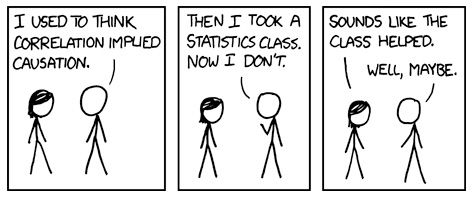
\includegraphics[scale=0.5]{figures/xkcd_correlation.jpg} \\
\end{center}
\begin{itemize}
\item Questions?
\item Introductions!
\end{itemize}
\end{frame}

\end{document}
